%% LaTeX Beamer presentation template (requires beamer package)
%% see http://bitbucket.org/rivanvx/beamer/wiki/Home
%% idea contributed by H. Turgut Uyar
%% template based on a template by Till Tantau
%% this template is still evolving - it might differ in future releases!

\documentclass{beamer}

\mode<presentation>
{
\usetheme{Warsaw}

\setbeamercovered{transparent}
}

\usepackage[english]{babel}
\usepackage[latin1]{inputenc}

% font definitions, try \usepackage{ae} instead of the following
% three lines if you don't like this look
\usepackage{mathptmx}
\usepackage[scaled=.90]{helvet}
\usepackage{courier}
\usepackage{xcolor}

\usepackage{amstext} % for \text macro
\usepackage{array}   % for \newcolumntype macro
\newcolumntype{L}{>{$}l<{$}} % math-mode version of "l" column type
\newcolumntype{C}{>{$}c<{$}} % math-mode version of "c" column type


\usepackage[T1]{fontenc}


\title[Predictive Active Steering Control for Autonomous Vehicle
Systems]{Example for an Model Predictive Controller
\\
for an active steering control  \\
of an automomous vehicle}

%\subtitle{}

% - Use the \inst{?} command only if the authors have different
%   affiliation.
\author{Dominique Laurencelle\inst{1} \and Stefan Glaser\inst{2}}
%\author{\inst{1}}

% - Use the \inst command only if there are several affiliations.
% - Keep it simple, no one is interested in your street address.
\institute[Universities of]
{
\inst{1}%
M.Sc. ESE\\
Albert Ludwigs University, Freiburg
\and
\inst{2}%
M.Sc. Informatics\\
Albert Ludwigs University, Freiburg}

\date{19.7.2016 / OMPC Seminar}


% This is only inserted into the PDF information catalog. Can be left
% out.
\subject{Talks}



% If you have a file called "university-logo-filename.xxx", where xxx
% is a graphic format that can be processed by latex or pdflatex,
% resp., then you can add a logo as follows:

% \pgfdeclareimage[height=0.5cm]{university-logo}{university-logo-filename}
% \logo{\pgfuseimage{university-logo}}



% Delete this, if you do not want the table of contents to pop up at
% the beginning of each subsection:
\AtBeginSubsection[]
{
\begin{frame}<beamer>
\frametitle{Outline}
\tableofcontents[currentsection,currentsubsection]
\end{frame}
}

% If you wish to uncover everything in a step-wise fashion, uncomment
% the following command:

%\beamerdefaultoverlayspecification{<+->}

\begin{document}

\begin{frame}
\titlepage
\end{frame}

% \begin{frame}
% \frametitle{Outline}
% \tableofcontents
% % You might wish to add the option [pausesections]
% \end{frame}


%============================================================
%=========================== LIPM ===========================
%============================================================
%\section*{Section name}

%\subsection*{Subsection1 name}
%\subsection*{Subsection2 name}

% \begin{frame}
% \frametitle{Motivation}
% 
% \begin{columns}[t,onlytextwidth]
% \column{.5\textwidth}
% Some motivation here
% 
% \column{.5\textwidth}
% or here
% 
% \end{columns}
% 
% \end{frame}





\begin{frame}
\frametitle{System Overview}

\begin{figure} [h]
\begin{center}
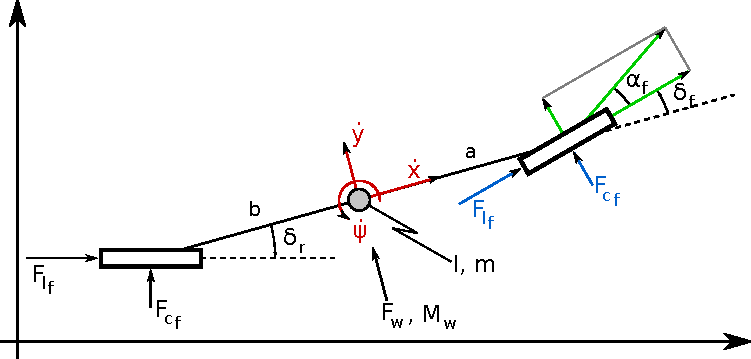
\includegraphics[scale=0.8]{images/dynamics_overview.pdf}
\label{fig:system_dynamics}
\end{center}
\end{figure}
% \[F_l : \text{Longitudial (tractive) force [N]} \qquad F_c : \text{Lateral
% (cornering) force [N]}\]
\[F_l, F_c : \text{Longitudial (tractive), lateral (cornering) force [N]}\]
% \[v_l : \text{Longitudial (tractive) velocity [m/s]} \qquad v_c : \text{Lateral
% (cornering) velocity [m/s]}\]
\[v_l, v_c : \text{Longitudial (tractive), lateral (cornering) velocity [m/s]}\]
\[\dot{x}, \dot{y} : \text{local velocities [m/s]} \qquad \dot{\psi} :
\text{angular velocity [1/s]}\]
\[\delta : \text{Steering angle [rad]} \qquad \alpha : \text{Slip angle [rad]}\]

\end{frame}





\begin{frame}
\frametitle{System overview}

% \begin{align*}
% v_{y_f} &= \dot{y} + a \dot{\psi}, & v_{y_r} &= \dot{y} - b \dot{\psi} \\
% v_{x_f} &= \dot{x}, & v_{x_r} &= \dot{x}
% \end{align*}
\begin{block}{System state and input}
\[\xi = [\dot{x}, \dot{y}, \psi, \dot{\psi}, X, Y] \qquad \qquad u = \delta_f \qquad \delta_r = 0\]
\end{block}

\begin{columns}[t,onlytextwidth]
\column{.45\textwidth}
\begin{block}{Vehicle dynamics}
\begin{align*}
\ddot{x} &= \dot{y} \dot{\psi} + \frac{2}{m} (F_{x_f} + F_{x_r}) \\
\ddot{y} &= - \dot{x} \dot{\psi} + \frac{2}{m} (F_{y_f} + F_{y_r}) \\
\ddot{\psi} &= \frac{2}{I} (a F_{y_f} - b F_{y_r}) \\
\dot{X} &= \dot{x} \ cos \psi - \dot{y} \ sin \psi \\
\dot{Y} &= \dot{x} \ sin \psi + \dot{y} \ cos \psi
\end{align*}
\end{block}

\column{.45\textwidth}
\begin{block}{Forces (front and rear wheels)}
\begin{align*}
F_x &= F_l \ cos \delta - F_c \ sin \delta \\
F_y &= F_l \ sin \delta + F_c \ cos \delta
\end{align*}
Pacejka tire model:
\begin{align*}
F_l &= f_l(\alpha, s, F_z) \\
F_c &= f_c(\alpha, s, F_z)
\end{align*}
\end{block}

\end{columns}

\end{frame}





\begin{frame}
\frametitle{Pacejka tire model}

\begin{figure} [h]
\begin{center}
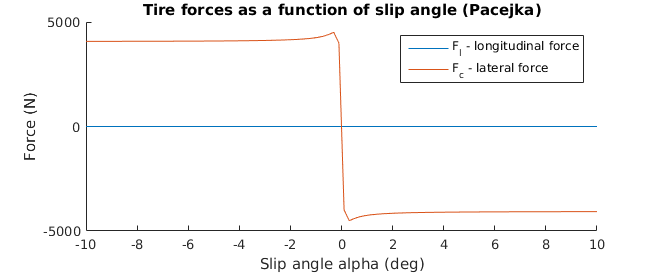
\includegraphics[scale=0.55]{images/pacejka_graph.png}
\label{fig:pacejka}
\end{center}
\end{figure}

\end{frame}





\begin{frame}
\frametitle{Trajectory generation}

\begin{align*}
Y_{ref}(X) &= 2.025 \ (1 + tanh(z_1)) - 2.85 \ (1 + tanh(z_2)) \\
\psi_{ref}(X) &= tan^{-1} \left( 0.1944 \ \left(\frac{1}{cosh(z_1)}\right)^2 - 0.311 \ \left(\frac{1}{cosh(z_2)}\right)^2 \right)
\end{align*}
\[\quad \text{with} \quad z_1 = \frac{2.4}{25}(X - 27.19) - 1.2 \qquad z_2 =
\frac{2.4}{21.95}(X - 56.46) - 1.2 \]


\begin{columns}[t,onlytextwidth]
\column{.5\textwidth}
\begin{figure} [h]
\begin{center}
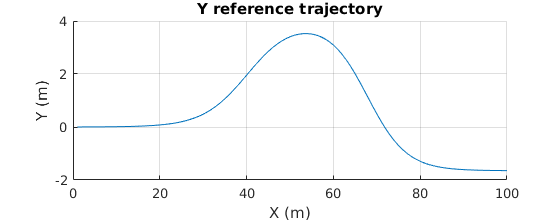
\includegraphics[scale=0.37]{images/Yref_graph.png}
\label{fig:y_reference}
\end{center}
\end{figure}

\column{.5\textwidth}
\begin{figure} [h]
\begin{center}
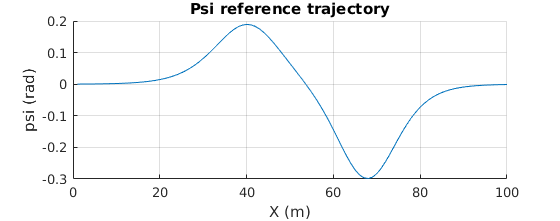
\includegraphics[scale=0.37]{images/Psiref_graph.png}
\label{fig:psi_reference}
\end{center}
\end{figure}

\end{columns}

\end{frame}





\begin{frame}
\frametitle{Trajectory generation}

\begin{figure} [h]
\begin{center}
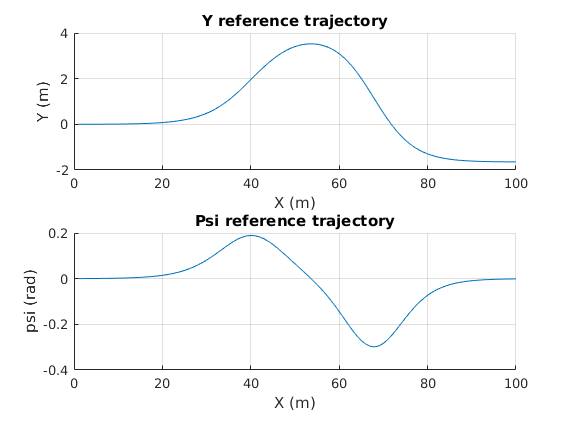
\includegraphics[scale=0.6]{images/trajectory_graph.png}
\label{fig:reference_trajectory}
\end{center}
\end{figure}

\end{frame}






\begin{frame}
\frametitle{Optimization problem}

\begin{block}{Objective function}


\begin{align*}
J(\xi_{t}, \Delta U_t) = &\sum_{i=1}^{H_p} ( ||\xi_{t+i,t}(6) -
Y_{ref_{t+i,t}}(\xi_{t+i,t}(5)) ||_{75}^2 \\ 
&+ ||\xi_{t+i,t}(3) -
\psi_{ref_{t+i,t}}(\xi_{t+i,t}(5)) ||_{500}^2 ) \\
&+ \sum_{i=0}^{H_c-1} || \Delta u_{t+i,t} ||_{150}^2
\end{align*}
\[\text{with} \quad H_p : \text{prediction horizon} \qquad H_c : \text{control
horizon}\]


\end{block}

\end{frame}







\begin{frame}
\frametitle{NLP problem formulation}

\begin{align*}
\min_{\Delta U_t \in \mathbb{R}^{H_p}} \quad &J(\xi_t, \Delta U_t) \\
s.t. \qquad &\xi_{k+1,t} = f(\xi_{k,t}, u_{k,t}) \\
&u_{k,t} = u_{k-1,t} + \Delta {u_{k,t}} \qquad \qquad k = t, . . . , t
+ H_{p}\\
&\delta_{min} \leq u_{k,t} \leq \delta_{max} \\
&\Delta \delta_{min} \leq \Delta u_{k,t} \leq \Delta \delta_{max} \qquad \quad k = t, . . . , t + H_c
-1 \\
&\Delta u_{k,t} = 0, \qquad \qquad k = t + H_c, . . . , t + H_p \\
&\xi_0 = \xi_{init} \\
& u_{-1} = u_{init}
\end{align*}

\end{frame}







\begin{frame}
\frametitle{LTV problem formulation }

\begin{align*}
\min_{\Delta U_t \in \mathbb{R}^{H_p}, \epsilon \in \mathbb{R}} \quad &J(\xi_t, \Delta U_t) +
\rho \epsilon \\
s.t. \qquad &\xi_{k+1,t} = A_t \xi_k + B_t u_k \\
&\alpha_{k,t} = C_t \xi_k + D_t u_k \\
&\alpha_{min} - \epsilon \leq \alpha_{k,t} \leq \alpha_{max} + \epsilon \\
&u_{k,t} = u_{k-1,t} + \Delta u_{k,t} \qquad \qquad k = t, . . . , t + H_p \\
&\delta_{min} \leq u_{k,t} \leq \delta_{max} \\ 
&\Delta \delta_{min} \leq \Delta u_{k,t} \leq \Delta \delta_{max} \qquad \qquad k = t, . . ., t + H_c - 1 \\
&\Delta u_k = 0, \qquad \qquad k = t + H_c, . . . , t + H_p \\
&\epsilon \geq 0 \\
&\xi_0 = \xi_{init} \\
& u_{-1} = u_{init}
\end{align*}

\end{frame}









\begin{frame}
\frametitle{Results}

\begin{center}
  \begin{tabular}{ |C|L|L|L|L| }
    \hline
    \textbf{5 m / s} & \multicolumn{4}{c|}{NL-MPC} \\ \hline
    H_p / H_c   & Y_{rms} & Y_{max} & \psi_{rms} & \psi_{max} \\ \hline
    3 \ / \ 3   & 0.004 & 0.216 & 0.543 & 1.987 \\ \hline
    7 \ / \ 3   & 0.001 & 0.084 & 0.274 & 1.356 \\ \hline
    15 \ / \ 10 & 3.991 * 10^{-4} & 0.055 & 0.399 & 1.666 \\ \hline
    25 \ / \ 10 & 1.001 * 10^{-4} & 0.0311 & 0.340 & 1.339 \\ \hline
  \end{tabular}
\end{center}

\begin{center}
  \begin{tabular}{ |C|L|L|L|L| }
    \hline
    \textbf{5 m / s} & \multicolumn{4}{c|}{LTV-MPC} \\ \hline
    H_p / H_c   & Y_{rms} & Y_{max} & \psi_{rms} & \psi_{max} \\ \hline
    3 \ / \ 3   & 0.005 & 0.206 & 1.595 & 4.716 \\ \hline
    7 \ / \ 3   & 0.020 & 0.398 & 2.119 & 3.479 \\ \hline
    15 \ / \ 10 & 0.050 & 0.593 & 3.468 & 4.592 \\ \hline
    25 \ / \ 10 & 0.073 & 0.728 & 4.336 & 5.188 \\ \hline
  \end{tabular}
\end{center}

\end{frame}






\begin{frame}
\frametitle{Results}

\begin{center}
  \begin{tabular}{ |C|L|L|L|L| }
    \hline
    \textbf{10 m / s} & \multicolumn{4}{c|}{NL-MPC} \\ \hline
    H_p / H_c   & Y_{rms} & Y_{max} & \psi_{rms} & \psi_{max} \\ \hline
    3 \ / \ 3   & 0.024 & 0.395 & 0.320 & 1.678 \\ \hline
    7 \ / \ 3   & 5.990*10^{-4} & 0.060 & 0.413 & 1.605 \\ \hline
    15 \ / \ 10 & 0.001 & 0.167 & 0.463 & 2.023 \\ \hline
    25 \ / \ 10 & 0.002 & 0.138 & 0.281 & 1.655 \\ \hline
  \end{tabular}
\end{center}

\begin{center}
  \begin{tabular}{ |C|L|L|L|L| }
    \hline
    \textbf{10 m / s} & \multicolumn{4}{c|}{LTV-MPC} \\ \hline
    H_p / H_c   & Y_{rms} & Y_{max} & \psi_{rms} & \psi_{max} \\ \hline
    3 \ / \ 3   & 0.003 & 0.149 & 2.093 & 3.671 \\ \hline
    7 \ / \ 3   & 0.099 & 0.815 & 5.234 & 5.558 \\ \hline
    15 \ / \ 10 & 0.158 & 0.977 & 6.700 & 6.460 \\ \hline
    25 \ / \ 10 & 0.193 & 1.051 & 7.161 & 6.735 \\ \hline
  \end{tabular}
\end{center}

\end{frame}






\begin{frame}
\frametitle{Results}

\begin{center}
  \begin{tabular}{ |C|L|L|L|L| }
    \hline
    \textbf{20 m / s} & \multicolumn{4}{c|}{NL-MPC} \\ \hline
    H_p / H_c   & Y_{rms} & Y_{max} & \psi_{rms} & \psi_{max} \\ \hline
    3 \ / \ 3   & 0.078 & 0.790 & 7.800 & 7.994 \\ \hline
    7 \ / \ 3   & 0.027 & 0.447 & 2.510 & 3.246 \\ \hline
    15 \ / \ 10 & 1.091*10^{3} & 7.198*10 & 2.982*10^{3} & 1.124*10^{2} \\ \hline
    25 \ / \ 10 & 1.275*10^{3} & 7.331*10 & 3.654*10^{3} & 1.245*10^{2} \\
    \hline
  \end{tabular}
\end{center}

\begin{center}
  \begin{tabular}{ |C|L|L|L|L| }
    \hline
    \textbf{20 m / s} & \multicolumn{4}{c|}{LTV-MPC} \\ \hline
    H_p / H_c   & Y_{rms} & Y_{max} & \psi_{rms} & \psi_{max} \\ \hline
    3 \ / \ 3   & 1.229*10^{2} & 3.371*10 & 1.063*10^{3} & 7.779*10^{2} \\
    \hline 7 \ / \ 3   & 0.360 & 1.616 & 1.306*10 & 9.754 \\ \hline
    15 \ / \ 10 & 7.162*10 & 2.741*10 & 7.706*10^2 & 6.944*10 \\ \hline
    25 \ / \ 10 & 0.329 & 1.456 & 1.011*10 & 65.174 \\ \hline
  \end{tabular}
\end{center}

\end{frame}


% \begin{frame}
% \frametitle<presentation>{Summary}
% 
% \begin{itemize}
%   \item The \alert{first main message} of your talk in one or two lines.
% \end{itemize}
% 
% % The following outlook is optional.
% \vskip0pt plus.5fill
% \begin{itemize}
%   \item Outlook
%   \begin{itemize}
%     \item Something you haven't solved.
%     \item Something else you haven't solved.
%   \end{itemize}
% \end{itemize}
% \end{frame}

\end{document}
